\documentclass[tikz,border=4pt]{standalone}
% Shared setup for the foundation-model diagrams, in the AFRICAST palette
\usepackage{fontspec}
\usepackage[sfdefault]{FiraSans}
\usepackage{amsmath}
\usepackage{unicode-math}
\setmathfont{Fira Math}
\usetikzlibrary{arrows.meta}
\definecolor{ink}{HTML}{1F2A36}
\definecolor{MonashBlue}{HTML}{3B75AC}
\definecolor{Orange}{HTML}{B5570F}
\color{ink}
\tikzset{every picture/.style={draw=ink,>=stealth}}
\hyphenpenalty=10000
\exhyphenpenalty=10000

\begin{document}
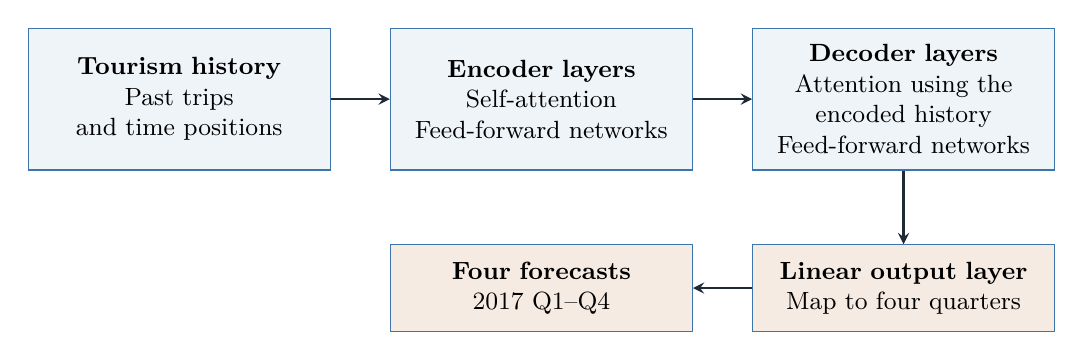
\begin{tikzpicture}[>=stealth,every node/.style={font=\fontsize{9}{11}\selectfont,align=center},
box/.style={draw=MonashBlue,fill=MonashBlue!8,text width=3.6cm,minimum height=1.8cm}]
\node[box] (data) at (0,0) {\textbf{Tourism history}\\Past trips\\and time positions};
\node[box] (enc) at (4.6,0) {\textbf{Encoder layers}\\Self-attention\\Feed-forward networks};
\node[box] (dec) at (9.2,0) {\textbf{Decoder layers}\\Attention using the\\encoded history\\Feed-forward networks};
\node[box,fill=Orange!12,minimum height=1.1cm] (linear) at (9.2,-2.4) {\textbf{Linear output layer}\\Map to four quarters};
\node[box,fill=Orange!12,minimum height=1.1cm] (pred) at (4.6,-2.4) {\textbf{Four forecasts}\\2017 Q1--Q4};
\draw[->,thick](data)--(enc);\draw[->,thick](enc)--(dec);
\draw[->,thick](dec)--(linear);\draw[->,thick](linear)--(pred);
\end{tikzpicture}
\end{document}
